% !TEX TS-program = pdflatex
% !TEX encoding = UTF-8 Unicode

% This is a simple template for a LaTeX document using the "article" class.
% See "book", "report", "letter" for other types of document.

\documentclass[12pt]{article} % use larger type; default would be 10pt

\usepackage[utf8]{inputenc} % set input encoding (not needed with XeLaTeX)

%%% Examples of Article customizations
% These packages are optional, depending whether you want the features they provide.
% See the LaTeX Companion or other references for full information.

%%% PAGE DIMENSIONS
\usepackage{geometry} % to change the page dimensions
\geometry{letterpaper} % or letterpaper (US) or a5paper or....
% \geometry{margin=2in} % for example, change the margins to 2 inches all round
% \geometry{landscape} % set up the page for landscape
%   read geometry.pdf for detailed page layout information

\usepackage{graphicx} % support the \includegraphics command and options

% \usepackage[parfill]{parskip} % Activate to begin paragraphs with an empty line rather than an indent

%%% PACKAGES
\usepackage{booktabs,tabularx} % for much better looking tables
\usepackage{array} % for better arrays (eg matrices) in maths
\usepackage{paralist} % very flexible & customisable lists (eg. enumerate/itemize, etc.)
\usepackage{verbatim} % adds environment for commenting out blocks of text & for better verbatim
\usepackage{subfig} % make it possible to include more than one captioned figure/table in a single float
% These packages are all incorporated in the memoir class to one degree or another...

%%% HEADERS & FOOTERS
\usepackage{fancyhdr} % This should be set AFTER setting up the page geometry
\usepackage[section]{placeins} % TO PREVENT FIGURES FROM BEING AFTER NEW SECTIONS
\pagestyle{fancy} % options: empty , plain , fancy
\renewcommand{\headrulewidth}{0pt} % customise the layout...
\lhead{}\chead{}\rhead{}
\lfoot{}\cfoot{\thepage}\rfoot{}

%%% SECTION TITLE APPEARANCE
\usepackage{sectsty}
\allsectionsfont{\sffamily\mdseries\upshape} % (See the fntguide.pdf for font help)
% (This matches ConTeXt defaults)

%%% ToC (table of contents) APPEARANCE
\usepackage[nottoc,notlof,notlot]{tocbibind} % Put the bibliography in the ToC
\usepackage[titles,subfigure]{tocloft} % Alter the style of the Table of Contents
\usepackage{amsmath,amssymb}
\usepackage{scrextend}
\usepackage{indentfirst}
\usepackage{changepage,titlesec}
\usepackage{xfrac}
\usepackage[T1]{fontenc}
\usepackage{float}
\renewcommand{\cftsecfont}{\rmfamily\mdseries\upshape}
\renewcommand{\cftsecpagefont}{\rmfamily\mdseries\upshape} % No bold!

% ---- To show code ---- (command \begin{lstlisting})
\usepackage{listings}
\usepackage{color}

\definecolor{dkgreen}{rgb}{0,0.6,0}
\definecolor{gray}{rgb}{0.5,0.5,0.5}
\definecolor{mauve}{rgb}{0.58,0,0.82}

\lstset{frame=tb,
  language=Java,
  aboveskip=3mm,
  belowskip=3mm,
  showstringspaces=false,
  columns=flexible,
  basicstyle={\small\ttfamily},
  numbers=none,
  numberstyle=\tiny\color{gray},
  keywordstyle=\color{blue},
  commentstyle=\color{dkgreen},
  stringstyle=\color{mauve},
  breaklines=true,
  breakatwhitespace=true,
  tabsize=3
}
%---

%%% END Article customizations

%%% The "real" document content comes below...
\renewcommand{\thesubsubsection}{\thesubsection.\alph{subsubsection}}
\titleformat{\subsubsection}[runin]% runin puts it in the same paragraph
        {\normalfont\bfseries}% formatting commands to apply to the whole heading
        {\thesubsubsection}% the label and number
        {0.5em}% space between label/number and subsection title
        {}% formatting commands applied just to subsection title
        []% punctuation or other commands following subsection title
\titlespacing*{\subsubsection} {1.2em}{2.25ex plus 1ex minus .2ex}{1em}
\newcolumntype{Y}{>{\raggedright\arraybackslash}X} 

\begin{document}
%% PAGE DE PRÉSENTATION %%
\begin{center}
	\thispagestyle{empty}
	\parskip=14pt%
	\vspace*{3\parskip}%
	Projet 1 \\
	IFT3913
	\bigbreak\bigbreak\bigbreak\bigbreak\bigbreak\bigbreak
	Olivier Hassaoui St-Amour (20078289)\\
	Francis Boulet-Rouleau (20067884)\\
	\bigbreak\bigbreak\bigbreak\bigbreak\bigbreak\bigbreak
	4 octobre 2018
\end{center}
\newpage

\section{Conception}
Pour ce projet, nous avons décidé d'adopter une conception MVC (Modèle-Vue-Controlleur) pour le déveleppement de l'application.  Le but était séparer les éléments de l'interface des éléments de logique pour pouvoir gérer les deux de la façon la plus indépendante possible.  Le constructeur étant utilisé comme pont entre le modèle et la vue.  Ainsi, le constructeur recevrait des requêtes de la vue demandant des informations du modèle.  Le constructeur demanderait ensuite au modèle de générer les données demandées et les retournerais à la vue pour les afficher.  Voici le diagramme de classe qui illustre la conception.
\begin{figure}[h]
  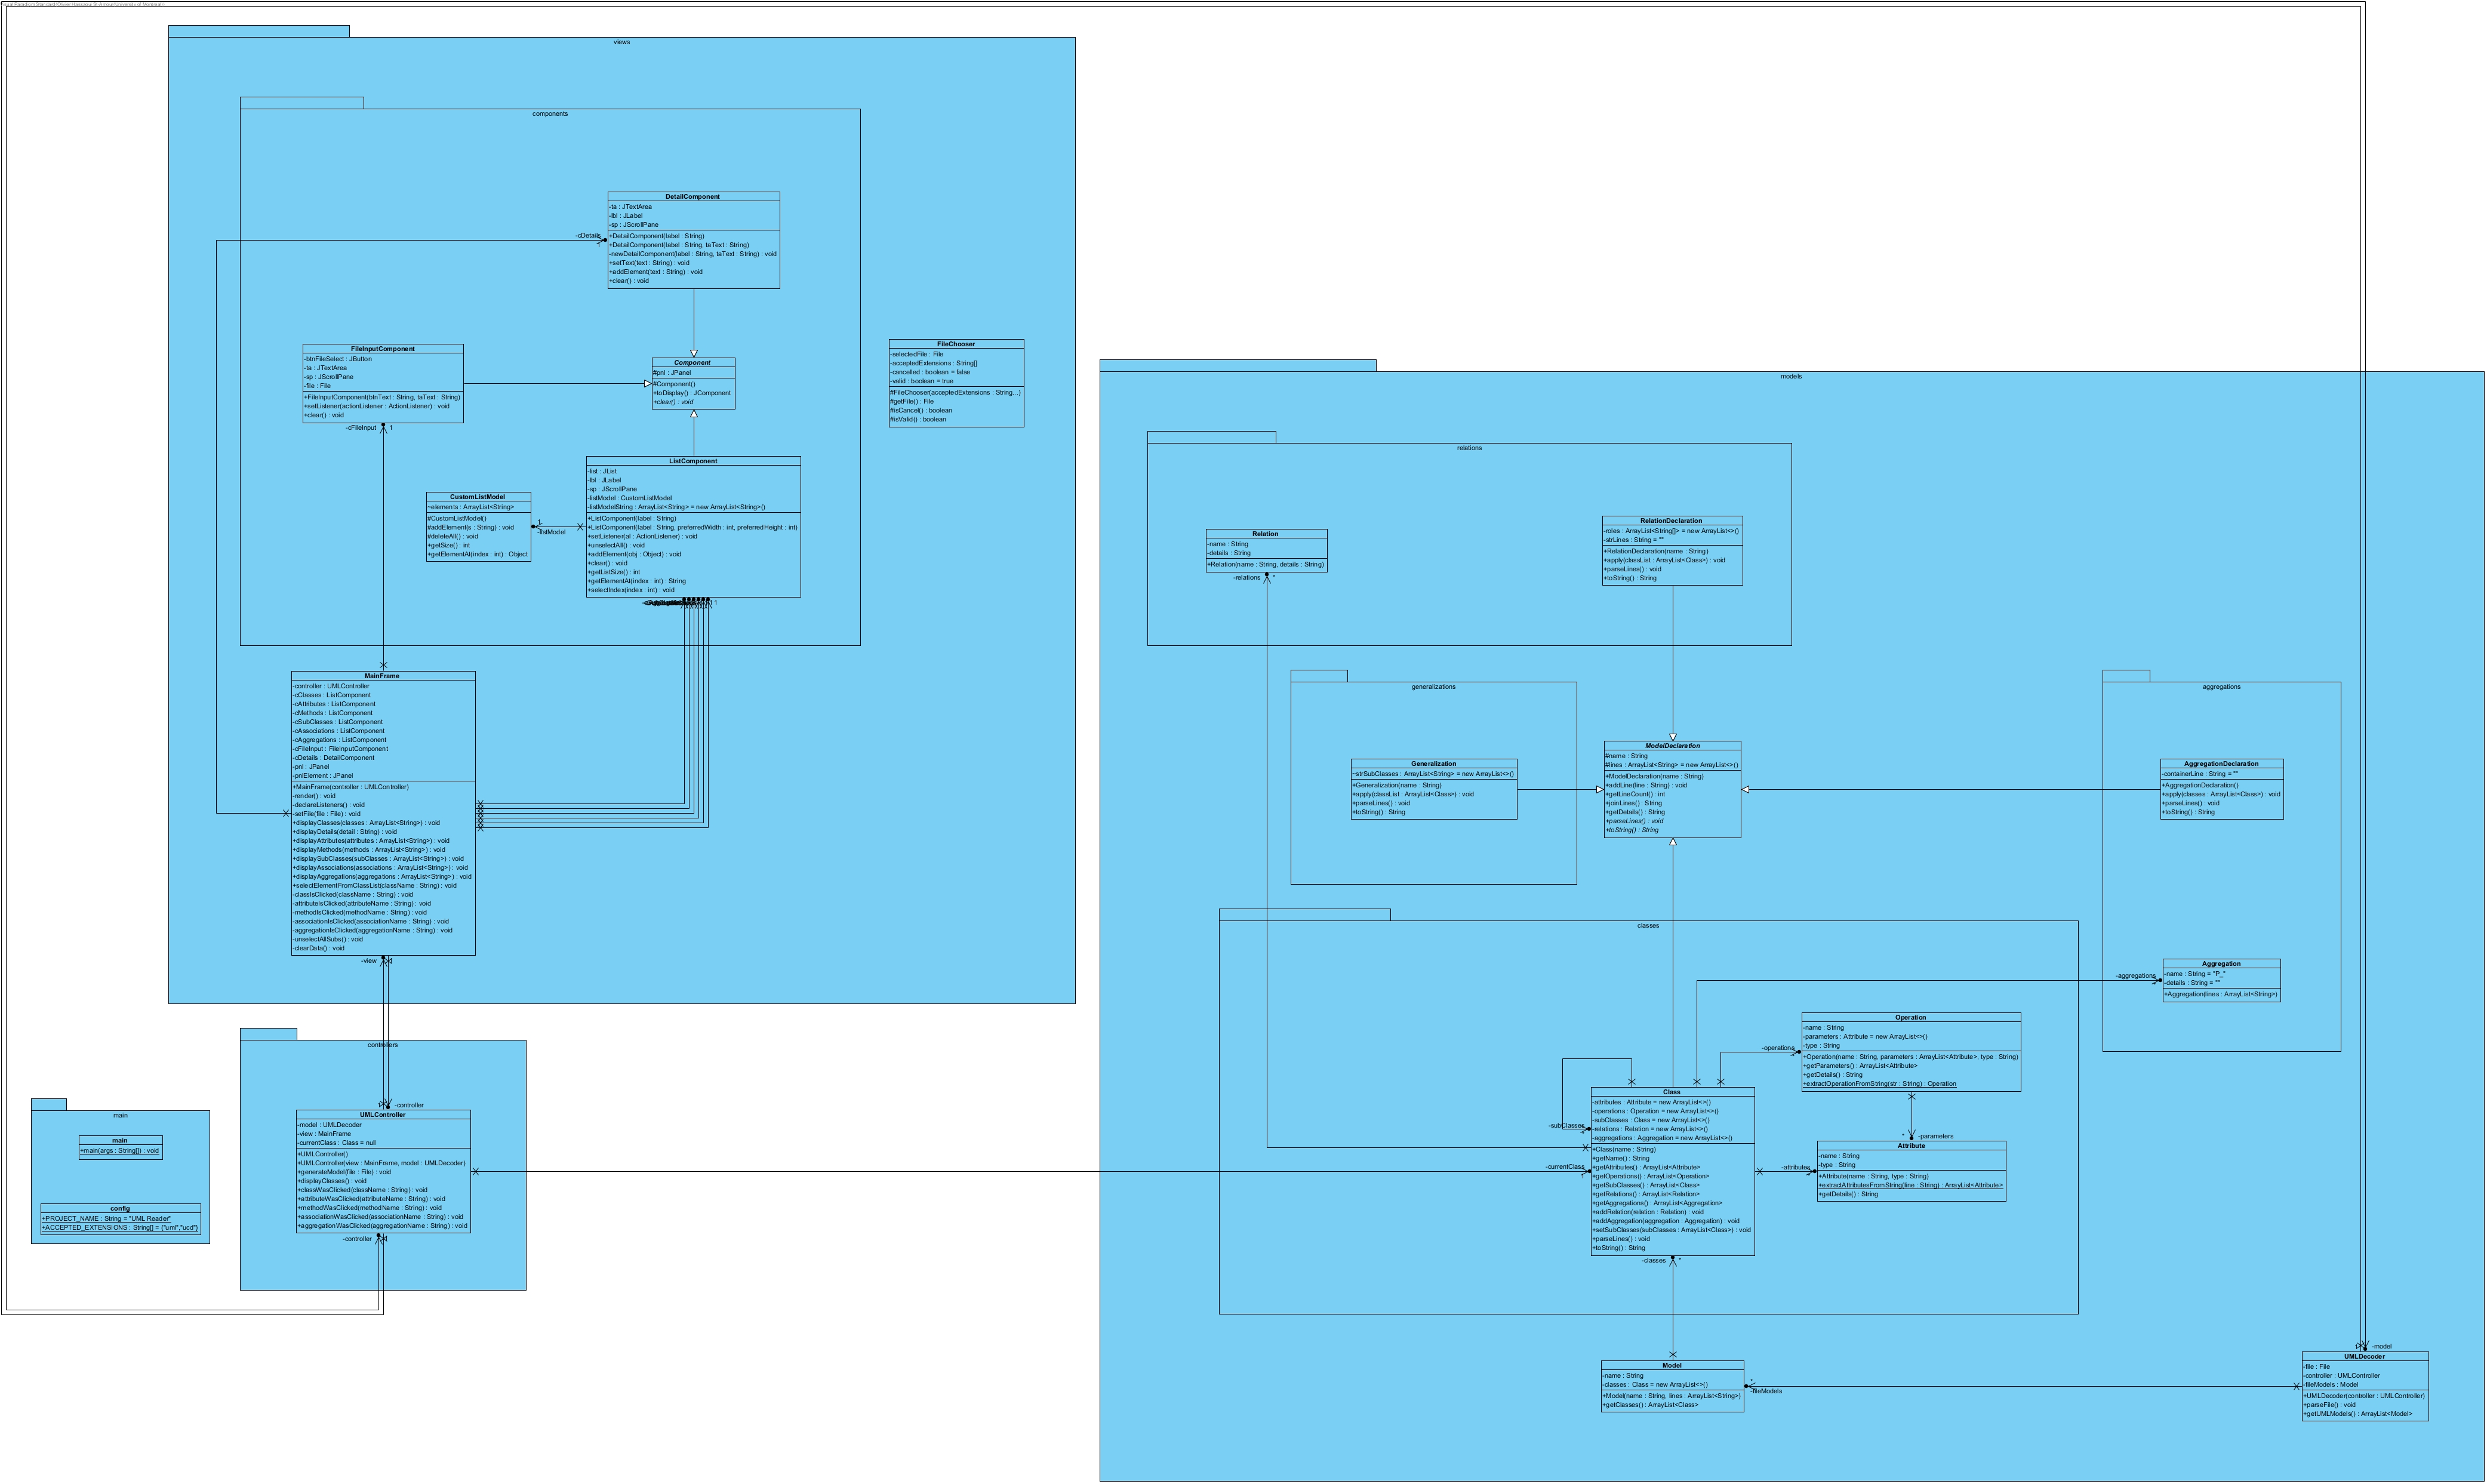
\includegraphics[width=\linewidth]{img/ClassDiagram.jpg}
  \label{fig:classdiagram}
\end{figure}

Les versions aggrandies de chacune des composantes du projet sont inclues dans les pages suivantes.  Pour permettre une meilleure visuallisation, un fichier .jpeg est remis avec le projet.

\begin{figure}[h]
  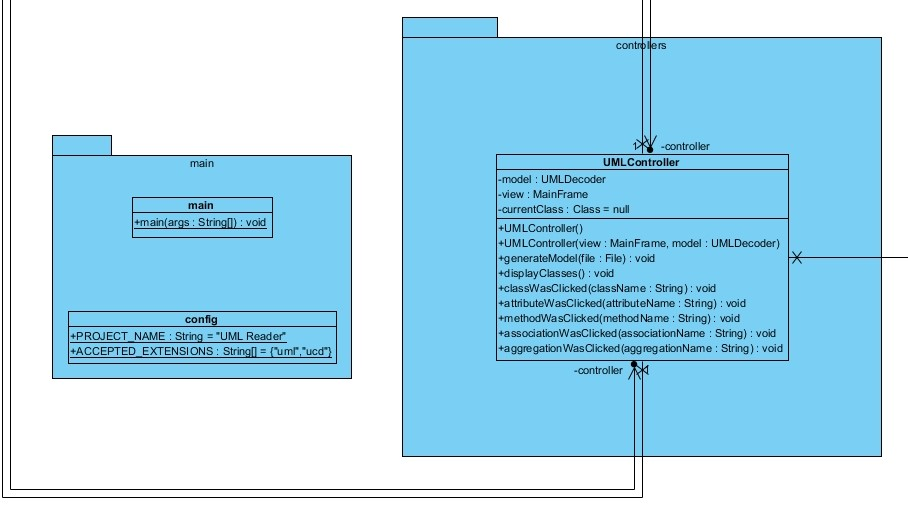
\includegraphics[width=\linewidth]{img/ClassDiagram-Controller.jpg}
  \caption{Diagramme de classe partielle représentant le point d'entré et le controlleur.}
  \label{fig:classdiagram-controller}
\end{figure}

\begin{figure}[h]
  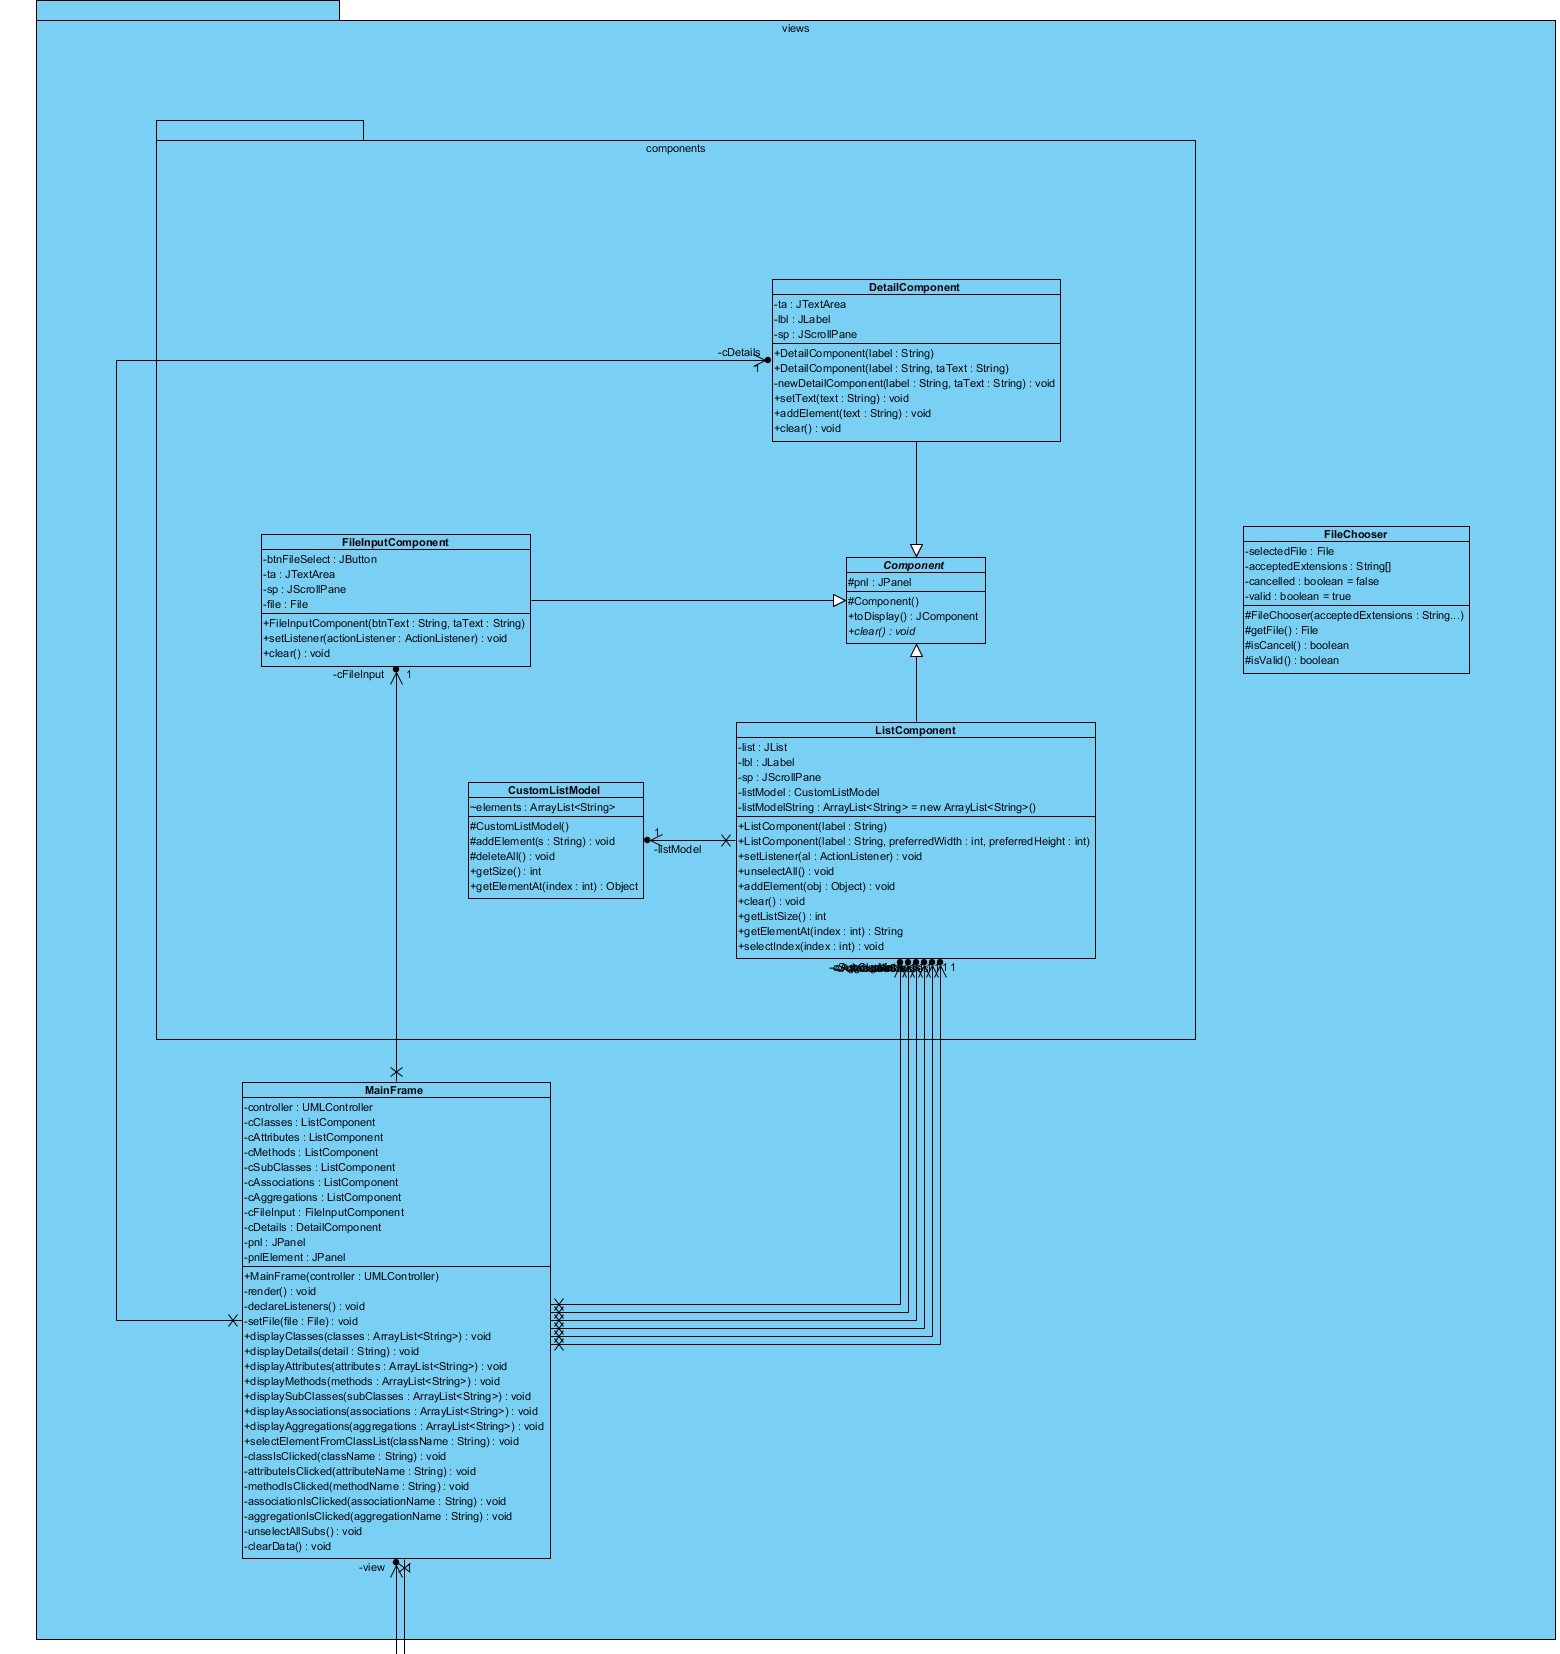
\includegraphics[width=\linewidth]{img/ClassDiagram-View.jpg}
  \caption{Diagramme de classe partielle représentant la vue.}
  \label{fig:classdiagram-view}
\end{figure}
\begin{figure}[h]
  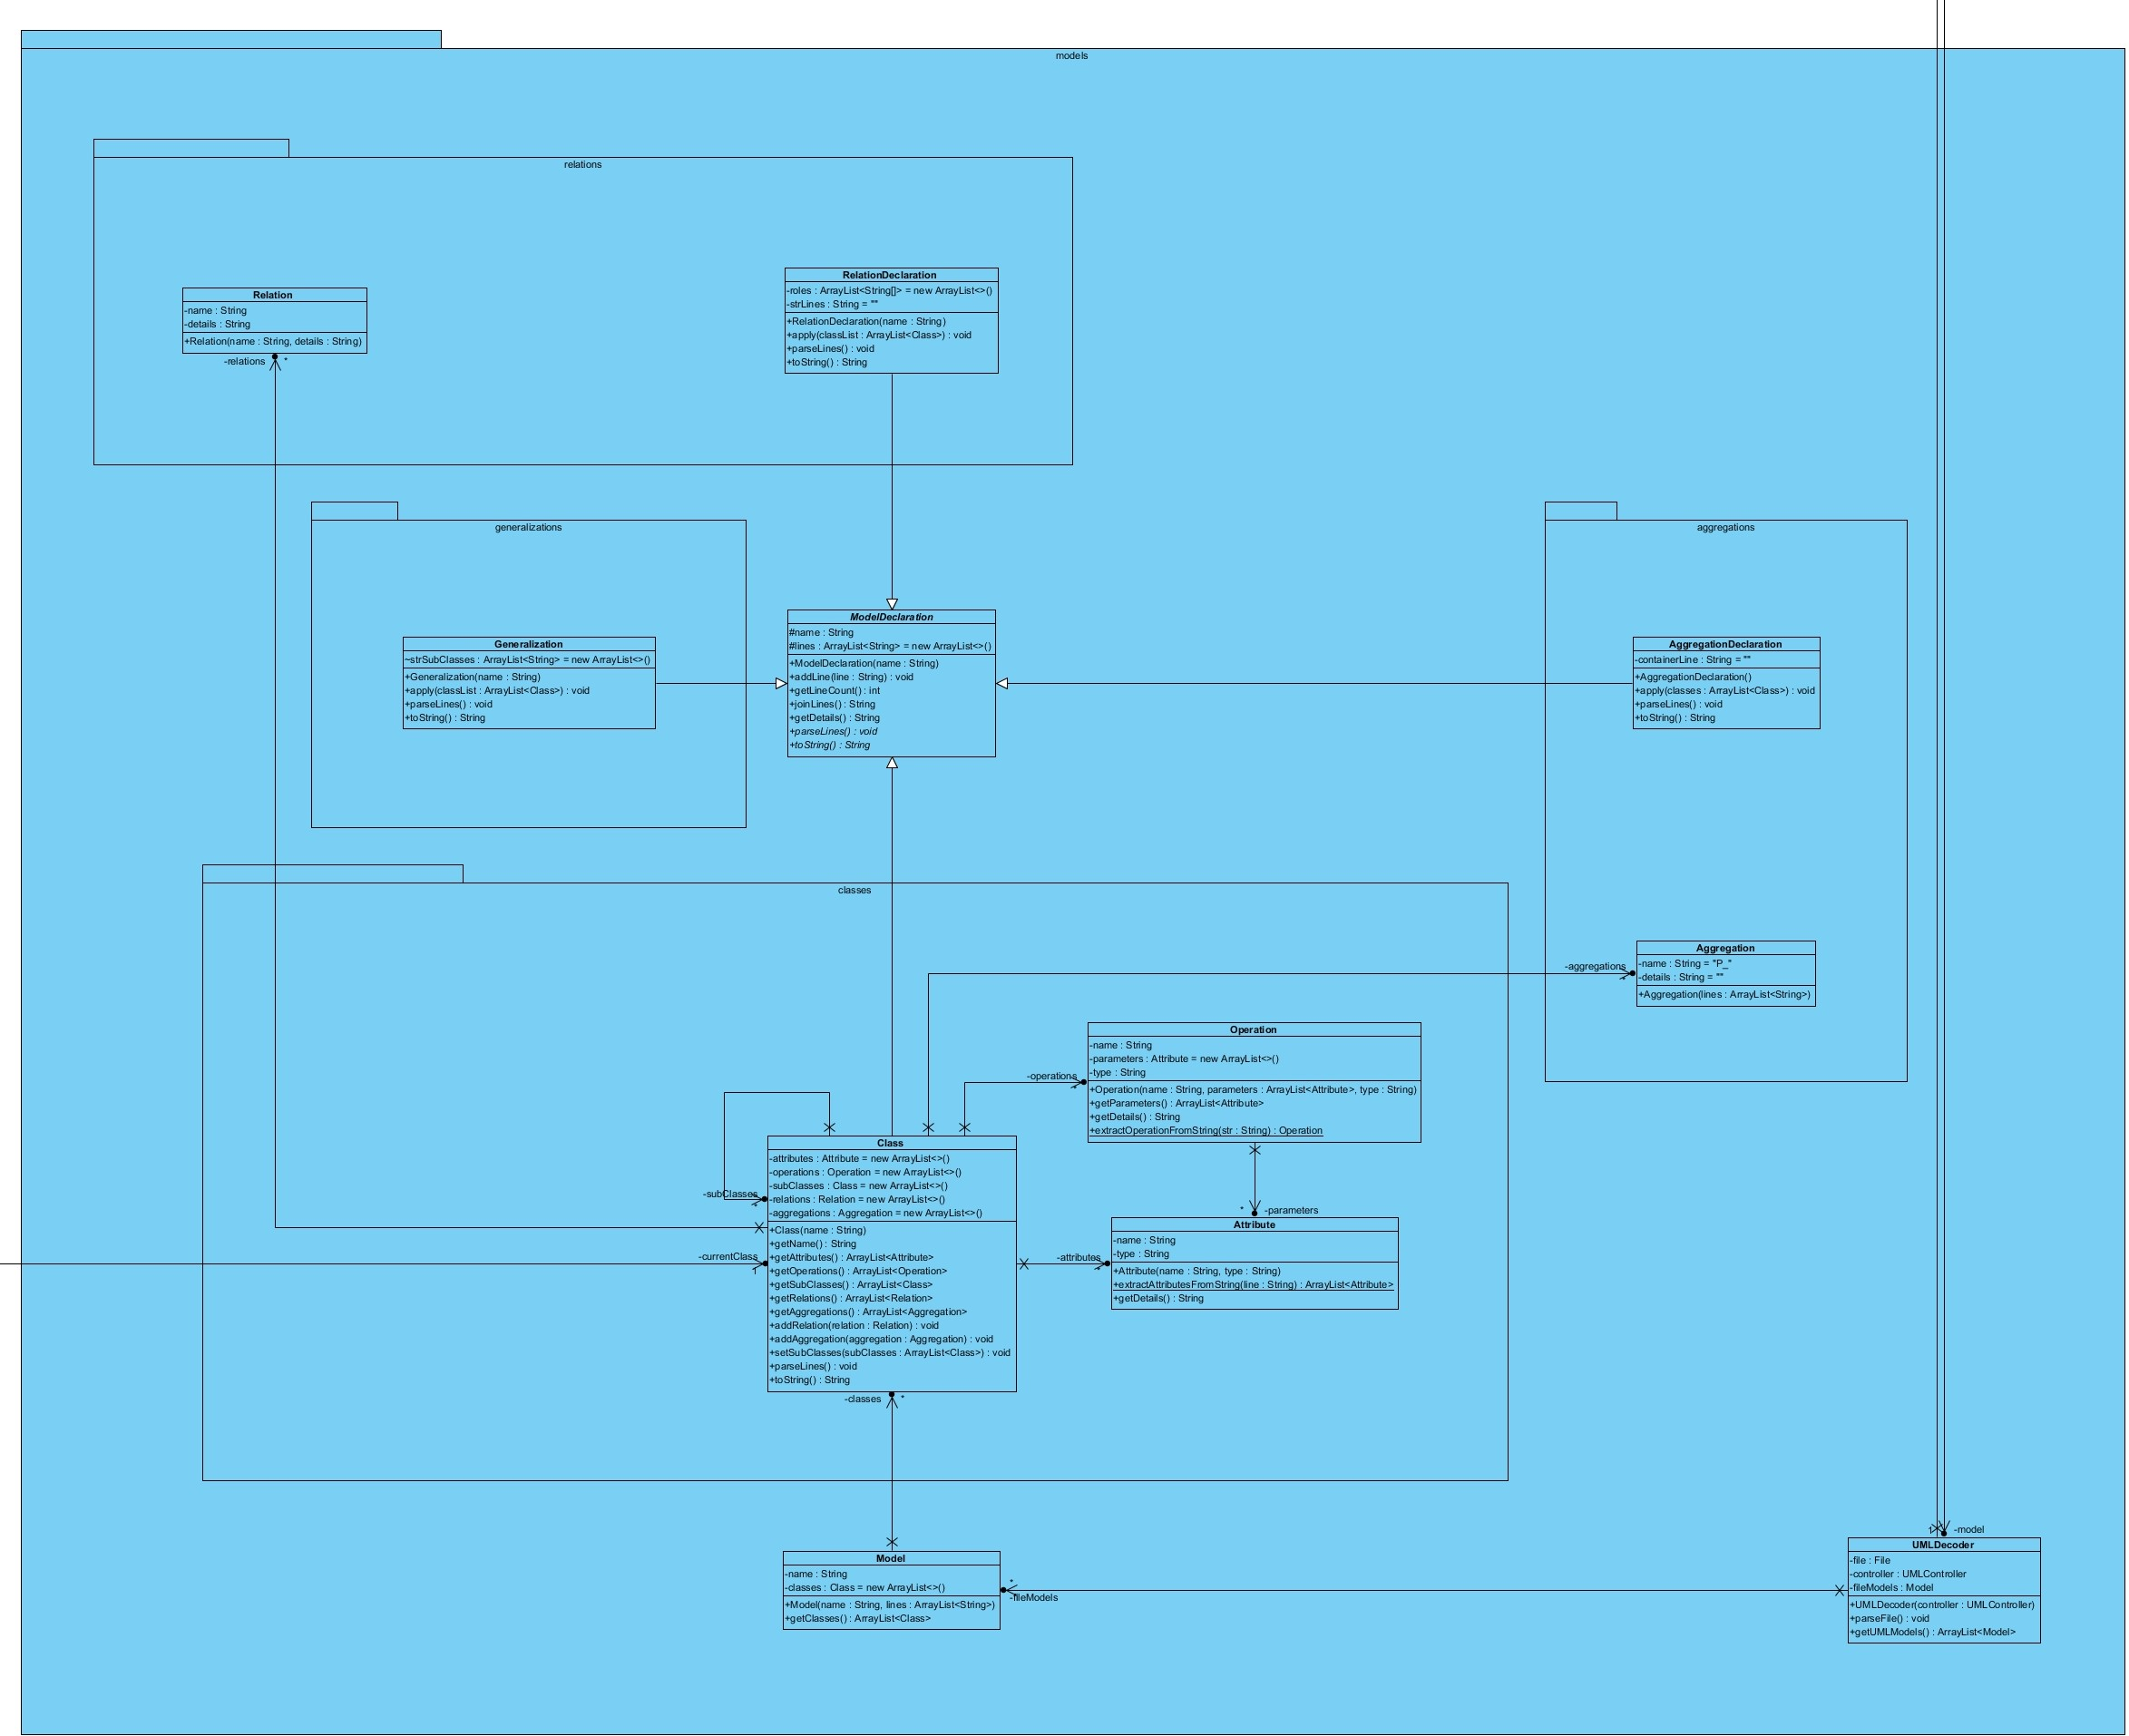
\includegraphics[width=\linewidth]{img/ClassDiagram-Model.jpg}
  \caption{Diagramme de classe partielle représentant le modèle.}
  \label{fig:classdiagram-model}
\end{figure}

\section{Implémentation}
Lors de l'implémentation, nous avons utiliser une approche qui priorisait l'encapsulation pour permettre une meilleure lisibilité de code et une maintenance de celui-ci plus facile.

\subsection{Modèle}
Pour la partie du modèle, son point d'entrée est la classe \textit{UMLDecoder} qui lit une première fois le fichier donné et y trouve tous les modèles UML qui s'y trouve.  Par la suite, il crée le nombre d'instances de \textit{Model} correspondant au nombre de modèles UML lus.  La classe \textit{Model} lit les lignes de caractères qui lui sont données et cherche dans ceux-ci les mots-clés qui indiquent la déclaration d'un nouvel élément UML.  Chacun des élément a une classe propre et le role de chaque classe est de \textit{parser} les lignes qui lui est donnée et populer ces différents attributs.  Une liste de \textit{Class} est ainsi générée pour que le controlleur puisse l'utiliser pour populer la vue.

Nous avons tenté de réduire le plus possible la duplication de code dans ce projet.  De ce fait, les classes \textit{Attribute} est utiliser à deux moments différents : pour définir les attributs de \textit{Class} et pour définir les attributs de \textit{Operation}.  Dans le même ordre d'idée, la classe \textit{Class} est utilisé premièrement pour instancier les classes UML et deuixièmement pour instancier les sous-classes de chacune des classes UML.

Pour l'instant, les spécifications expliquaient qu'il n'y aurait qu'un modèle par fichier.  Cependant, le modèle est fait de sorte à lire plus qu'un modèle s'il y en a plusieurs de définis dans le fichier.

Il est à noté que le \textit{parsing} se base de façon importante sur le format UML.  Par exemple, lorsqu'on croise le mot-clé ''ATTRIBUTES'', le parseur examine la ligne suivante pour trouver les attributs de la classe.  Ainsi, si les attributs se trouvent sur la même ligne que le mot-clé, ils sont ignorés par le parseur.


\subsection{Vue}
L'outil d'interfrace utilisé pour ce projet est la libraire \textit{Swing}. 

Le point d'entrée de la partie vue est la classe \textit{MainFrame}.  Lors de son instanciation, la vue crée d'abord toutes les composantes requises sans y afficher de données (évidemment).  Les composantes sont créé grâce à la classe abstraite \textit{Component}.  Cette classe sert à être héritée par les autres composantes d'affichage.  C'est composantes sont \textit{FileInputComponent}, \textit{ListComponent} et \textit{DetailsComponent}.  Dans l'ordre, ils servent à :\\
\indent1. Créer un bouton suivi d'un champs texte pour le téléchargement de fichier.\\
\indent2. Créer une liste dans un \textit{ScrollPane} avec une étiquette au dessus.\\
\indent3. Créer une zone de texte non-éditable avec une étiquette au dessus.\\
Chacune de ces classes est requise d'avoir une fonction \textit{toDisplay()} qui peut être appelé lorsque l'on veut ajouter la composante à un \textit{JFrame}.

L'instance de \textit{MainFrame} utilise ensuite ces composantes pour construire l'interface suivante :

\begin{figure}[h]
  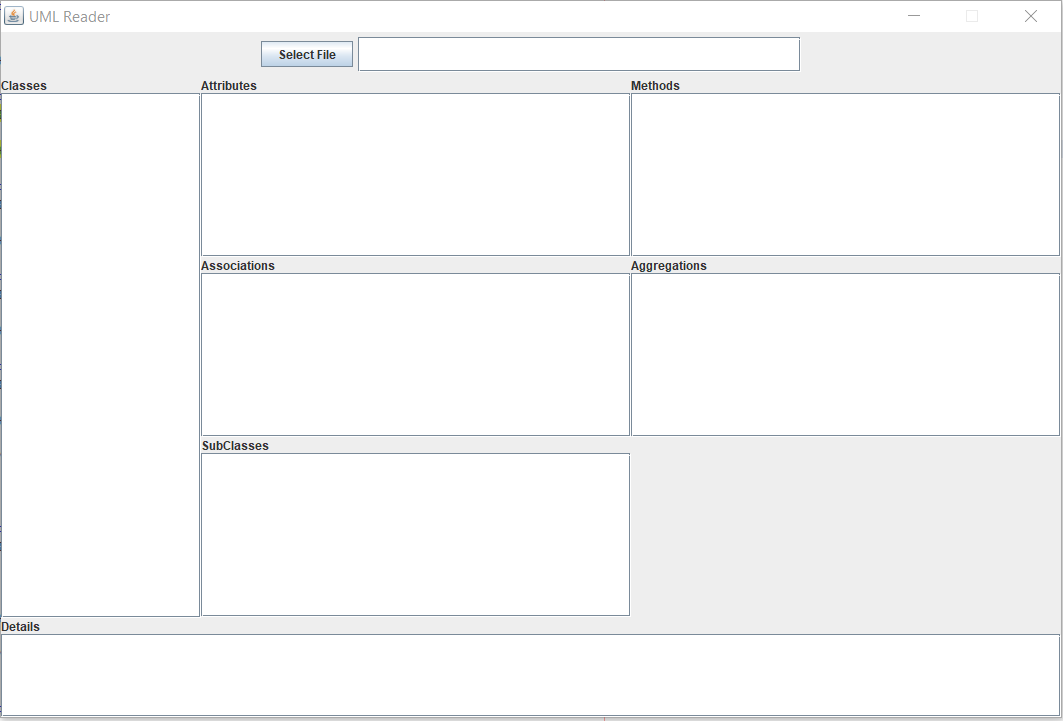
\includegraphics[width=\linewidth]{img/interface.PNG}
  \caption{Interface du projet de parseur UML}
  \label{fig:interface}
\end{figure}

Il est à noter que les \textit{Component} ne sont pas responsables de déclarer les actions que des interactions avec leurs éléments graphique produisent.  Ainsi, si on ajoute une composante \textit{FileInputComponent} à la fenêtre sans rien faire d'autre et qu'on clique ensuite sur le bouton de la composante, rien ne se produit, il faut spécifier que l'action effectuer lors du clique est la création d'une fenêtre de \textit{FileChooser}.  De ce fait, c'est la classe \textit{MainFrame} qui, lors de l'instanciation des \textit{Component}, leur lie explicitement des \textit{ActionListenent}, \textit{KeyListener}, etc.

\subsection{Gestion des erreurs}
La plupart des erreurs que le système est capable d'intercepter sont géré par la vue et le controlleur.  La vue s'occupe de s'assurer que le fichier fournit à la bonne extension et est non vide et le controlleur vérifie que le \textit{Model} généré n'a pas d'erreur.  En effet, si le fichier à la bonne extension et est non-vide, mais tout de même invalide, il est envoyé malgré tout à la classe \textit{UMLDecoder} qui, en cas de malformation, ne générera pas de donnés.  C'est ensuite au controlleur à vérifier que des données ont bel-et-bien été générées, sans quoi, il ordonne à la vue d'afficher un message d'erreur.

\section{Conclusion}
En bref, nous avons opté pour une conception MVC qui facilite la maintenance du projet en permettant une meilleure lecture du code et en permettant d'ajouter des fonctionnalités de façon relativement facile.  En effet, si un nouvel élément descriptif UML s'ajoute, il sera assez simple de l'inclure dans la partie Modèle et également simple dans la partie Vue.   Dans le Modèle, l'ajout demanderait la création d'une nouvelle classe pour décrire le nouvel élément et dans la Vue, il suffirait d'ajouter un \textit{Component} à l'interface.

Aussi, le couplage entre les composantes du projet est faible.  En effet, on peut modifier la Vue sans devoir changer quoi que ce soit au Modèle.  On peut aussi faire l'inverse avec modification relativement minime de la Vue.  Également, les éléments du Modèle sont également relativement indépendants entre eux, permettant de changer leur implementation individuelle sans affecter le comportement du programme en général.

\section{Manuel d'utilisateur}
L'interface montrée à la figure 4 est relativement instinctive à naviguer.  D'abord, il faut selectionner un fichier, puis, si le fichier est valide, une liste de classes s'affichera (sinon, un message d'erreur).  On peut ensuite naviguer à travers le modèle UML est double cliquant sur une classes, ce qui affichera ces attributs et autres éléments descriptifs dans les bons champs.  Chaque champs peut être double-cliqué pour afficher ces détails (s'il y en a).
\\

L'utilisation a été testée avec la version 1.8.0\_181 de Java (JRE) et le Java Development Kit (JDK) 1.8.0\_144
Les lignes de commandes pour démarer le projet sont les suivantes.
\begin{lstlisting}
cd ./$DIRECTORY/dist
java -jar UML_reader.jar
\end{lstlisting}
\end{document}
